\begin{bt}
Chứng minh rằng trong một hình bình hành, tổng bình phương hai đường chéo bằng tổng bình phương các cạnh.
\end{bt}
\begin{proof}
Xét hình bình hành $ABCD$ như sau:
\begin{center}
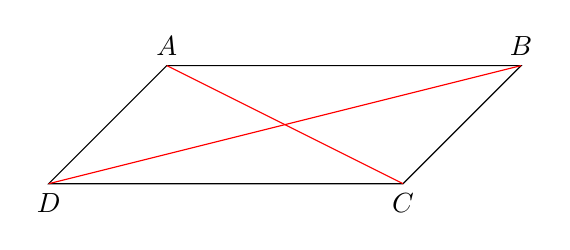
\begin{tikzpicture}[scale=1.5]
\draw[color=black] (0,0)node[above]{$A$}--(3,0)node[above]{$B$}--(2,-1)node[below]{$C$}--(-1,-1)node[below]{$D$}--(0,0);
\draw[color=red] (0,0)--(2,-1);
\draw[color=red] (3,0)--(-1,-1);
\end{tikzpicture}    
\end{center}
\begin{align*}
\text{Ta có: } AC^2+BD^2&=(\vt{AC})^2+(\vt{BD})^2=(\vt{AB}+\vt{BC})^2+(\vt{BC}+\vt{CD})^2\\
&=(\vt{AB})^2+(\vt{BC})^2+2.\vt{AB}.\vt{BC}+(\vt{BC})^2+(\vt{CD})^2+2.\vt{BC}.\vt{CD}\\
&=AB^2+BC^2 + CD^2+AD^2+ 2.\vt{BC}.\underbrace{(\vt{AB}+\vt{CD})} \\
& \hspace{7.5cm}\vt{0}
\end{align*}
Do đó, ta được $AC^2+BD^2=AB^2+BC^2 + CD^2+AD^2$ (đpcm).
\end{proof}
\end{tcolorbox}
